%\documentclass[handout]{beamer}
\documentclass[]{beamer}
%\usepackage[dvips]{color}
\usepackage{graphicx}
\usepackage{amsmath,amssymb,array,eucal,url}
\usepackage{xcolor}
\definecolor{beamer@blendedblue}{RGB}{86,155,189}
\definecolor{myblue}{RGB}{12,76,138}
\setbeamercolor{structure}{fg=myblue}
\definecolor{Ftitle}{RGB}{12,76,138}
\definecolor{Descitem}{RGB}{238,238,244}
\definecolor{StdTitle}{RGB}{12,76,138}
\definecolor{StdBody}{RGB}{213,24,0}
\definecolor{StdBody}{RGB}{213,24,0}

\definecolor{AlTitle}{RGB}{255, 190, 190}
\definecolor{AlBody}{RGB}{213,24,0}

\definecolor{ExTitle}{RGB}{201, 217, 217}
\definecolor{ExBody}{RGB}{213,24,0}

\setbeamercolor{frametitle}{fg = Ftitle}
\setbeamercolor{title}{fg = Ftitle}
\setbeamercolor{item}{fg = Ftitle}
\setbeamercolor{subitem}{fg = Ftitle}
\setbeamercolor{subsubitem}{fg = Ftitle}
\setbeamercolor{description item}{fg = myblue}
\setbeamercolor{titlelike}{fg=myblue}

\DeclareMathOperator{\sgn}{sgn}
\newcommand{\e}{\mathbf{e}}
\renewcommand{\P}{\mathbf{P}}
\newcommand{\F}{\mathbf{F}}
\newcommand{\R}{\textsf{R}}
\newcommand{\mat}[1] {\mathbf{#1}}
%\newcommand{\ind}{\mathrel{\mathop{\sim}\limits^{\mathit{ind}}}}
%\newcommand{\iid}{\mathrel{\mathop{\sim}\limits^{\mathit{iid}}}}
\newcommand{\E}{\textsf{E}}
\newcommand{\SE}{\textsf{SE}}
\newcommand{\SSE}{\textsf{SSE}}
\newcommand{\RSS}{\textsf{RSS}}
\newcommand{\FSS}{\textsf{FSS}}
\renewcommand{\SS}{\textsf{SS}}
\newcommand{\MSE}{\textsf{MSE}}
\newcommand{\SSR}{\textsf{SSR}}
\newcommand{\Be}{\textsf{Beta}}
\newcommand{\St}{\textsf{St}}
\newcommand{\Ca}{\textsf{C}}
\newcommand{\Exp}{\textsf{Exp}}
\newcommand{\GDP}{\textsf{GDP}}
\newcommand{\NcSt}{\textsf{NcSt}}
\newcommand{\Bin}{\textsf{Bin}}
\newcommand{\NB}{\textsf{NegBin}}
\renewcommand{\NG}{\textsf{NG}}
\newcommand{\N}{\textsf{N}}
\newcommand{\Ber}{\textsf{Ber}}
\newcommand{\Poi}{\text{Poi}}
\newcommand{\Gam}{\textsf{Gamma}}
\newcommand{\BB}{\textsf{BB}}
\newcommand{\Gm}{\textsf{G}}
\newcommand{\Un}{\textsf{Unif}}
\newcommand{\Ex}{\textsf{Exp}}
\newcommand{\DE}{\textsf{DE}}
\newcommand{\tr}{\textsf{tr}}
\newcommand{\cF}{{\cal{F}}}
\newcommand{\cL}{{\cal{L}}}
\newcommand{\cI}{{\cal{I}}}
\newcommand{\cB}{{\cal{B}}}
\newcommand{\cP}{{\cal{P}}}
\newcommand{\bbR}{\mathbb{R}}
\newcommand{\bbN}{\mathbb{N}}
\newcommand{\pperp}{\mathrel{{\rlap{$\,\perp$}\perp\,\,}}}
\newcommand{\OFP}{(\Omega,\cF, \P)}
\newcommand{\eps}{\boldsymbol{\epsilon}}
\newcommand{\1}{\mathbf{1}_n}
\newcommand{\gap}{\vspace{8mm}}
\newcommand{\ind}{\mathrel{\mathop{\sim}\limits^{\rm ind}}}
\newcommand{\simiid}{\ensuremath{\mathrel{\mathop{\sim}\limits^{\rm
iid}}}}
\newcommand{\eqindis}{\ensuremath{\mathrel{\mathop{=}\limits^{\rm D}}}}
\newcommand{\iid}{\textit{i.i.d.}}
\newcommand{\SSZ}{S_{zz}}
\newcommand{\SZW}{S_{zw}}
\newcommand{\Var}{\textsf{Var}}
\newcommand{\corr}{\textsf{corr}}
\newcommand{\diag}{\textsf{diag}}
\newcommand{\var}{\textsf{var}}
\newcommand{\Cov}{\textsf{Cov}}
\newcommand{\Sam}{{\cal S}}
\def\H{\mathbf{H}}
\newcommand{\I}{\mathbf{I}}
\newcommand{\Y}{\mathbf{Y}}
\newcommand{\tY}{\tilde{\mathbf{Y}}}
\newcommand{\Yhat}{\hat{\mathbf{Y}}}
\newcommand{\Yobs}{\mathbf{Y}_{{\cal S}}}
\newcommand{\barYobs}{\bar{Y}_{{\cal S}}}
\newcommand{\barYmiss}{\bar{Y}_{{\cal S}^c}}
\def\bv{\mathbf{b}}
\def\X{\mathbf{X}}
\def\tX{\tilde{\mathbf{X}}}
\def\x{\mathbf{x}}
\def\xbar{\bar{\mathbf{x}}}
\def\Xbar{\bar{\mathbf{X}}}
\def\Xg{\mathbf{X}_{\boldsymbol{\gamma}}}
\def\Ybar{\bar{\Y}}
\def\ybar{\bar{y}}
\def\y{\mathbf{y}}
\def\Yf{\mathbf{Y_f}}
\def\W{\mathbf{W}}
\def\L{\mathbf{L}}
\def\w{\mathbf{w}}
\def\U{\mathbf{U}}
\def\V{\mathbf{V}}
\def\Q{\mathbf{Q}}
\def\Z{\mathbf{Z}}
\def\z{\mathbf{z}}
\def\v{\mathbf{v}}
\def\u{\mathbf{u}}

\def\zero{\mathbf{0}}
\def\one{\mathbf{1}}
\newcommand{\taub}{\boldsymbol{\tau}}
\newcommand{\betav}{\boldsymbol{\beta}}
\newcommand{\alphav}{\boldsymbol{\alpha}}
\newcommand{\A}{\mathbf{A}}
\def\a{\mathbf{a}}
\def\K{\mathbf{K}}
\newcommand{\B}{\mathbf{B}}
\def\b{\boldsymbol{\beta}}
\def\bhat{\hat{\boldsymbol{\beta}}}
\def\btilde{\tilde{\boldsymbol{\beta}}}
\def\tb{\boldsymbol{\theta}}
\def\bg{\boldsymbol{\beta_\gamma}}
\def\bgnot{\boldsymbol{\beta_{(-\gamma)}}}
\def\mub{\boldsymbol{\mu}}
\def\tmub{\tilde{\boldsymbol{\mu}}}
\def\muhat{\hat{\boldsymbol{\mu}}}
\def\tb{\boldsymbol{\theta}}
\def\tk{\boldsymbol{\theta}_k}
\def\tj{\boldsymbol{\theta}_j}
\def\Mk{\boldsymbol{{\cal M}}_k}
\def\M{\boldsymbol{{\cal M}}}
\def\Mj{\boldsymbol{{\cal M}}_j}
\def\Mi{\boldsymbol{{\cal M}}_i}
\def\Mg{{\boldsymbol{{\cal M}_\gamma}}}
\def\Mnull{\boldsymbol{{\cal M}}_{N}}
\def\gMPM{\boldsymbol{\gamma}_{\text{MPM}}}
\def\gHPM{\boldsymbol{\gamma}_{\text{HPM}}}
\def\Mfull{\boldsymbol{{\cal M}}_{F}}
\def\tg{\boldsymbol{\theta}_{\boldsymbol{\gamma}}}
\def\g{\boldsymbol{\gamma}}
\def\eg{\boldsymbol{\eta}_{\boldsymbol{\gamma}}}
\def\G{\mathbf{G}}
\def\cM{\cal M}
\def\D{\Delta}
\def \shat{{\hat{\sigma}}^2}
\def\uv{\mathbf{u}}
\def\l {\lambda}
\def\d{\delta}
\def\Sigmab{\boldsymbol{\Sigma}}
\def\Lambdab{\boldsymbol{\Lambda}}
\def\lambdab{\boldsymbol{\lambda}}
\def\Mg{{\cal M}_\gamma}
\def\S{{\cal{S}}}
\def\qg{p_{\boldsymbol{\gamma}}}
\def\pg{p_{\boldsymbol{\gamma}}}
%\def\t{\mathbf{t}}
\def\T{\boldsymbol{\Theta}}
\def\Tb{\boldsymbol{\Theta}}
\def\t{\mathbf{t}}

\usepackage{verbatim}

\usetheme{default}

\title{Lasso \& Bayesian  Lasso }
\subtitle{Readings Chapter 15 Christensen}
\institute{Merlise Clyde}
\author{STA721 Linear Models Duke University}
\date{\today}
\logo{duke.eps}

\begin{document}
\maketitle


\begin{frame}
  \frametitle{Lasso}
Tibshirani (JRSS B 1996) proposed estimating coefficients through
$L_1$ constrained least squares  ``Least Absolute Shrinkage and
Selection Operator''
\begin{itemize}
 \item Control how large coefficients may grow \pause
    $$\min_{\b^s} (\Y^c - \X^s \b^s)^T (\Y^c - \X^s\b^s)$$
    subject to
    $$ \sum |\beta^s_j| \le t$$ \pause
  \item Equivalent Quadratic Programming Problem for ``penalized'' Likelihood
    $$\min_{\b} \| \Y^c - \X^s \b^s\|^2 + \lambda \|\b^s\|_1$$ \pause
  \item Posterior mode
  $$
\max_{\b^s} -\frac{\phi}{2} \{ \| \Y^c - \X^s \b^s\|^2 + \lambda^* \|\b^s\|_1 \}
$$
\end{itemize}
\end{frame}
\begin{frame}
  \frametitle{Picture}

\end{frame}
\begin{frame}[fragile]
  \frametitle{R Code}
The entire path of solutions can be easily found using the
   ``Least Angle Regression'' Algorithm of Efron et al (Annals of
   Statistics 2004)
\begin{verbatim}
> library(lars)
> longley.lars = lars(as.matrix(longley[,-7]), longley[,7],
                 type="lasso")
> plot(longley.lars)
\end{verbatim}
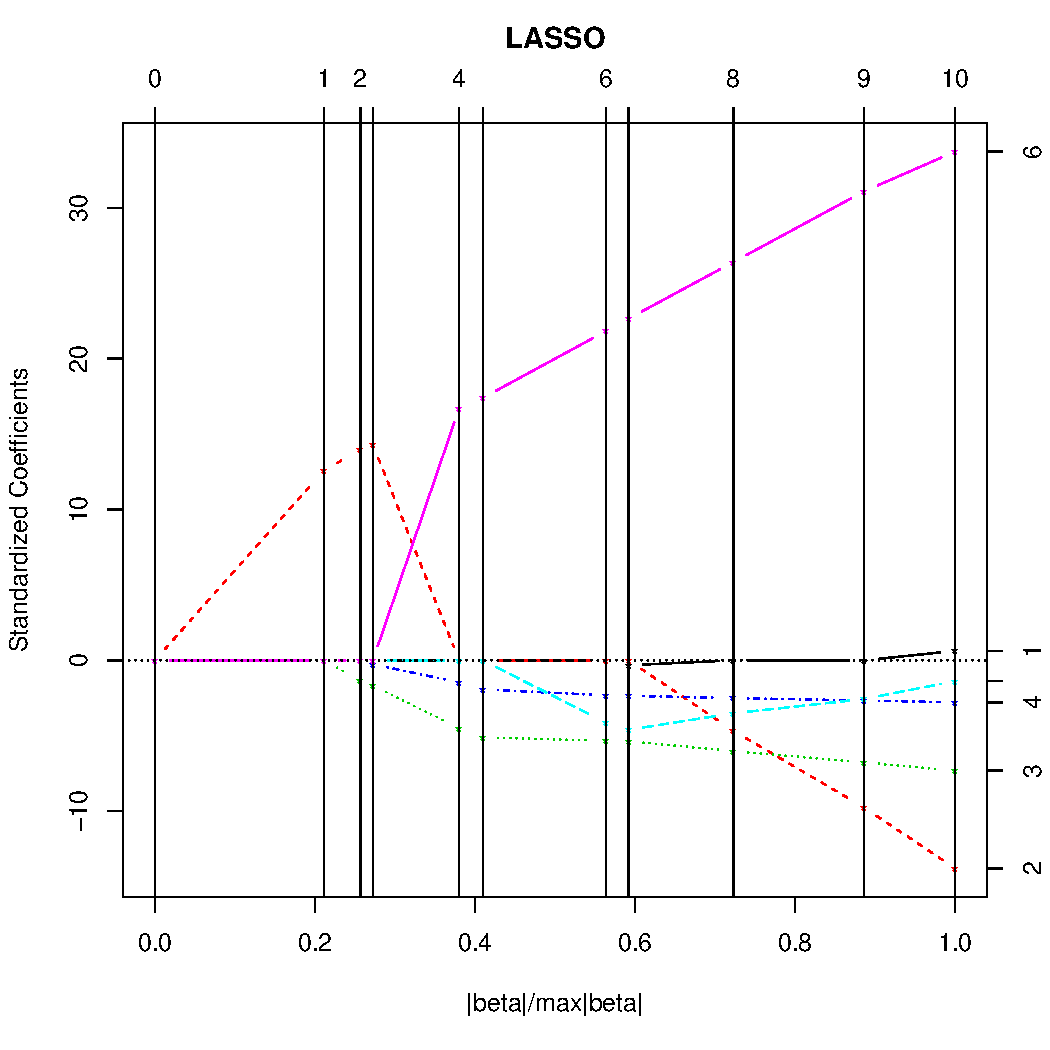
\includegraphics[height=2in]{longley-lars}
\end{frame}

\begin{frame}[fragile]
  \frametitle{Solutions}
{\fontsize{9pt}{10pt} \selectfont
\begin{verbatim}
> round(coef(longley.lars),5)
    GNP.deflator      GNP Unemployed Armed.Forces Population    Year
 [1,]    0.00000  0.00000    0.00000      0.00000    0.00000 0.00000
 [2,]    0.00000  0.03273    0.00000      0.00000    0.00000 0.00000
 [3,]    0.00000  0.03623   -0.00372      0.00000    0.00000 0.00000
 [4,]    0.00000  0.03717   -0.00459     -0.00099    0.00000 0.00000
 [5,]    0.00000  0.00000   -0.01242     -0.00539    0.00000 0.90681
 [6,]    0.00000  0.00000   -0.01412     -0.00713    0.00000 0.94375
 [7,]    0.00000  0.00000   -0.01471     -0.00861   -0.15337 1.18430
 [8,]   -0.00770  0.00000   -0.01481     -0.00873   -0.17076 1.22888
 [9,]    0.00000 -0.01212   -0.01663     -0.00927   -0.13029 1.43192
[10,]    0.00000 -0.02534   -0.01869     -0.00989   -0.09514 1.68655
[11,]    0.01506 -0.03582   -0.02020     -0.01033   -0.05110 1.82915
\end{verbatim}
}
\end{frame}

\begin{frame}[fragile]
  \frametitle{Cp Solution}
Min $C_p = SSE_p/\hat{\sigma}^2_F - n + 2 p$  \pause
\begin{small}
\begin{verbatim}
> summary(longley.lars)
LARS/LASSO
Call: lars(x = as.matrix(longley[, -7]), y = longley[, 7], type = "lasso")
   Df     Rss        Cp
0   1 185.009 1976.7120
1   2   6.642   59.4712
2   3   3.883   31.7832
3   4   3.468   29.3165
4   5   1.563   10.8183
5   4   1.339    6.4068
6   5   1.024    5.0186
7   6   0.998    6.7388
8   7   0.907    7.7615
9   6   0.847    5.1128
10  7   0.836    7.0000
\end{verbatim}
\end{small}
 \pause
{\fontsize{9pt}{10pt} \selectfont
\begin{verbatim}
     GNP.deflator     GNP Unemployed Armed.Forces Population    Year
[7,]     0.00000  0.00000   -0.01471     -0.00861   -0.15337 1.18430

\end{verbatim}
}

\end{frame}
\begin{frame}
  \frametitle{Features}
Combines shrinkage (like Ridge Regression) with Selection (like
stepwise selection) \pause

\vspace{24pt}
Uncertainty  in  penalty? \pause

\vspace{24pt}
Interval estimates?
\end{frame}
\begin{frame}
  \frametitle{Bayesian Lasso}
  Park \& Casella (JASA 2008) and Hans (Biometrika 2010) propose
  Bayesian versions of the Lasso  \pause
  \begin{eqnarray*}
    \Y \mid \alpha, \b^s, \phi & \sim & \N(\one_n \alpha + \X^s \b^s, \I_n/\phi)  \pause\\
    \b^s \mid \alpha, \phi, \taub & \sim & \N(\zero, \diag(\taub^2)/\phi)  \pause\\
    \tau_1^2 \ldots, \tau_p^2 \mid \alpha, \phi & \simiid & \Ex(\lambda^2/2)  \pause\\
    p(\alpha, \phi) & \propto& 1/\phi  \pause\\
  \end{eqnarray*}
Can show that $\beta_j \mid \phi, \lambda \simiid DE(\lambda \sqrt{\phi})$
$$\int_0^\infty \frac{1}{\sqrt{2 \pi s}}
  e^{-\frac{1}{2} \phi \frac{\beta^2}{s }}
  \, \frac{\lambda^2}{2} e^{- \frac{\lambda^2 s}{2}}\, ds =
  \frac{\lambda \phi^{1/2}}{2} e^{-\lambda \phi^{1/2} |\beta|}
$$  \pause
Scale Mixture of Normals  (Andrews and Mallows 1974)
\end{frame}
\begin{frame}
  \frametitle{Gibbs Sampling}
  \begin{itemize}
  \item Integrate out $\alpha$: $\alpha \mid \Y, \phi \sim \N(\ybar,
    1/(n \phi)$  \pause
\item $\b^s \mid \taub, \phi, \lambda, \Y \sim \N(, )$   \pause
\item $\phi \mid \taub, \b^s, \lambda, \Y \sim \G( , ) $  \pause
\item $1/\tau_j^2 \mid \b^s, \phi, \lambda, \Y \sim \text{InvGaussian}(
  , )$  \pause
  \end{itemize}
$X \sim \textsf{InvGaussian}(\mu,  \lambda)$
$$
f(x) =  \sqrt{\frac{\lambda^2}{2 \pi}}  x^{-3/2} e^{- \frac{1}{2} \frac{
    \lambda^2( x - \mu)^2} {\mu^2 x}} \qquad x > 0
$$  \pause

Homework:  Derive the full conditionals for $\b^s$, $\phi$,
$1/\tau^2$  see \url{http://www.stat.ufl.edu/~casella/Papers/Lasso.pdf}
\end{frame}
\begin{frame}
  \frametitle{Other Options}
  Range of other scale mixtures used  \pause
  \begin{itemize}
  \item Horseshoe  (Carvalho, Polson \& Scott)  \pause
  \item Generalized Double Pareto (Armagan, Dunson \& Lee)  \pause
  \item Normal-Exponenetial-Gamma (Griffen \& Brown)  \pause
  \item Bridge - Power Exponential Priors  \pause
   \end{itemize}
Properties of Prior?   \pause
\end{frame}








\begin{frame}
  \frametitle{Horseshoe}
  Carvalho, Polson \& Scott  propose
\begin{itemize}
\item
Prior Distribution on $$\b \mid \phi \sim \N(\zero_p, \frac{\diag(\tau^2)}{ \phi
    }) $$ \pause
\item $\tau_j^2 \mid \lambda \simiid C^+(0, \lambda)$ \pause
\item $\lambda \sim \Ca^+(0, 1/\phi)$ \pause
\item $p(\alpha, \phi) \propto 1/\phi)$ \pause
\end{itemize}

In the case $\lambda = \phi = 1$ and with $\X^t\X = \I$, $\Y^* =
\X^T\Y$ \pause
$$
E[\beta_i \mid \Y] = \int_0^1 (1 - \kappa_i) y^*_i p(\kappa_i \mid \Y)
\ d\kappa_i = (1 - \E[\kappa \mid y^*_i]) y^*_i$$
where $\kappa_i = 1/(1 + \tau_i^2)$ shrinkage factor \pause

\vspace{18pt}
Half-Cauchy prior induces a Beta(1/2, 1/2) distribution on $\kappa_i$
a priori
\end{frame}
\begin{frame}
\frametitle{Horseshoe}
  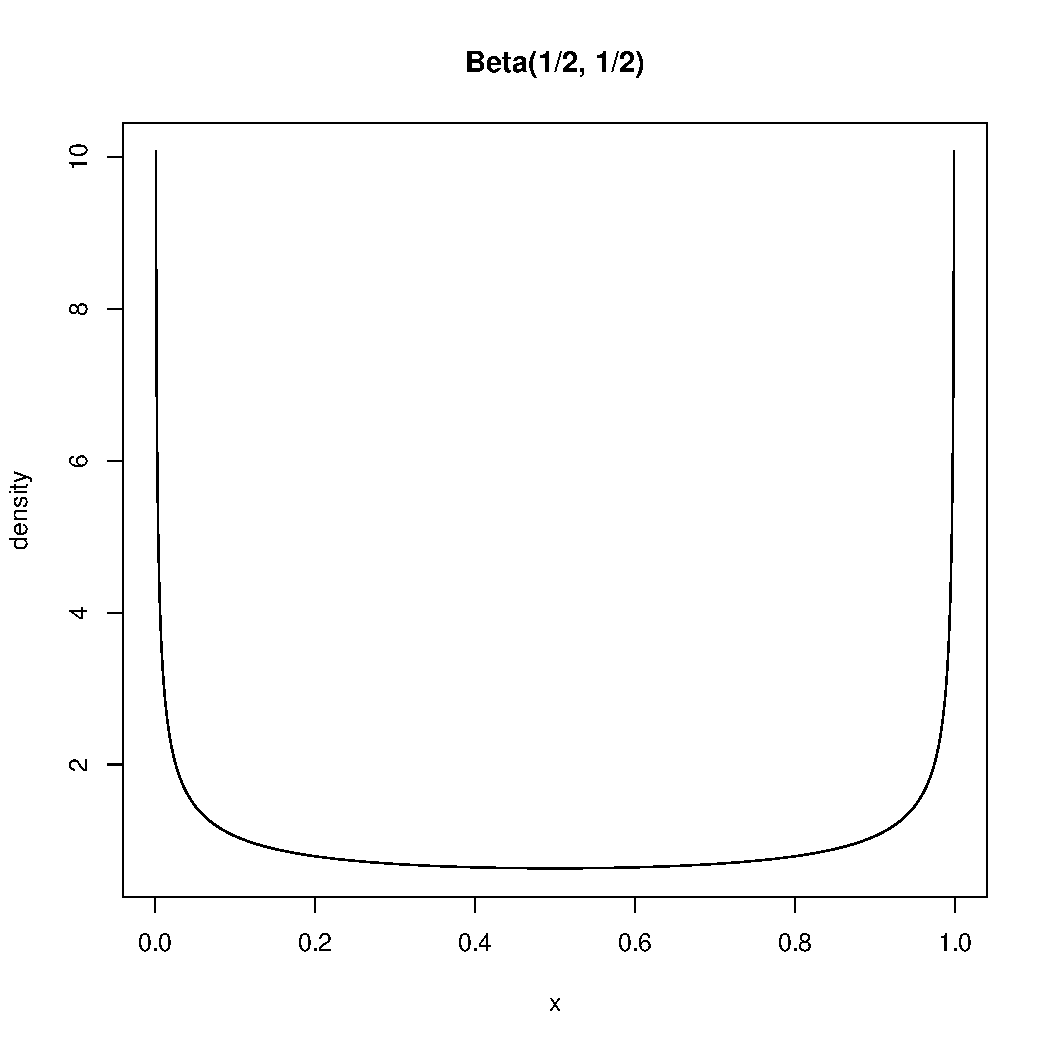
\includegraphics[height=3.5in]{beta}
\end{frame}



\begin{frame}
  \frametitle{Simulation Study with Diabetes Data}
  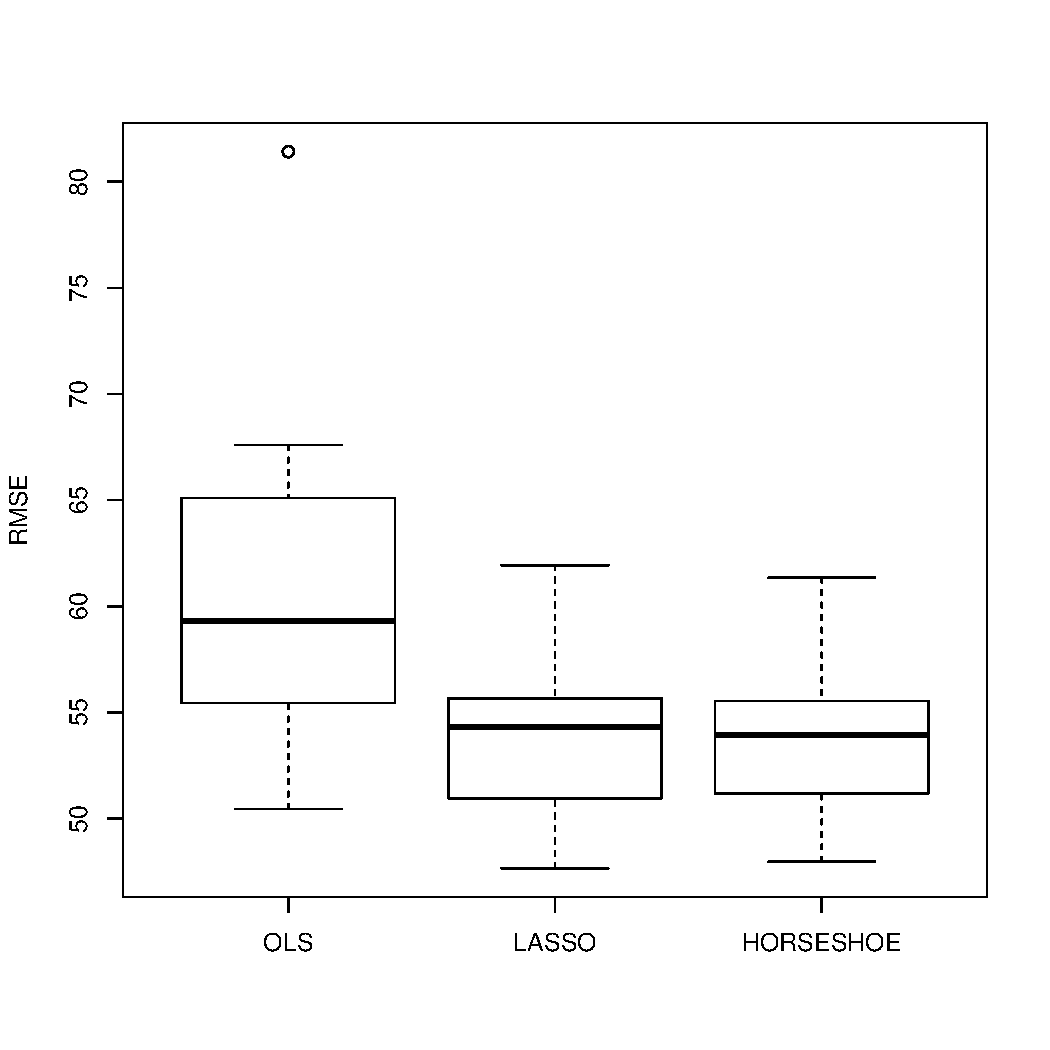
\includegraphics[height=3.5in]{diabetes}
\end{frame}

\begin{frame}
  \frametitle{Other Options}
  Range of other scale mixtures used  \pause
  \begin{itemize}
  \item Generalized Double Pareto (Armagan, Dunson \& Lee)  \pause
$\lambda \sim \Gam(\alpha, \eta)$  then $\beta_j \sim \textsf{GDP}(\xi
= \eta/\alpha, \alpha)$  \pause
$$
f(\beta_j) = \frac{1}{2 \xi} (1 + \frac{|\beta_j|}{\xi \alpha})^{-(1 + \alpha)}
$$

see \url{http://arxiv.org/pdf/1104.0861.pdf} \pause
  \item Normal-Exponenetial-Gamma (Griffen \& Brown 2005)
$\lambda^2 \sim \Gam(\alpha, \eta)$
  \pause
  \item Bridge - Power Exponential Priors  (Stable mixing density) \pause

   \end{itemize}
See the monomvn package on CRAN \pause

\vfill

Choice of prior?   Properties?  Fan \& Li (JASA 2001) discuss Variable
selection via nonconcave penalties and oracle properties
\end{frame}

\begin{frame}
  \frametitle{Choice of Estimator \& Selection?}

  \begin{itemize}
  \item Posterior Mode (may set some coefficients to zero) \pause
  \item Posterior Mean (no selection) \pause
  \end{itemize}
  Bayesian Posterior does not assign any probability to $\beta_j = 0$ \pause

  \begin{itemize}
  \item selection based on posterior mode ad hoc rule - Select if
    $\kappa_i < .5)$ \pause \\
See  article by  Datta \& Ghosh
\url{http://ba.stat.cmu.edu/journal/forthcoming/datta.pdf} \pause
  \item Selection solved as a post-analysis decision problem \pause
  \item Selection part of model uncertainty $\Rightarrow$ add prior \pause
    probability that $\beta_j = 0$  and combine with decision problem
  \end{itemize}
\end{frame}


\end{document}

